\documentclass[11pt,a4paper]{article}

\usepackage[utf8]{inputenc}
\usepackage[T1]{fontenc}
\usepackage{lmodern}
\usepackage{microtype}
\usepackage[margin=1in]{geometry}
\usepackage{setspace}
\onehalfspacing
\usepackage{graphicx}
\usepackage{booktabs}
\usepackage{siunitx}
\usepackage{tabularx}
\usepackage{xcolor}
\usepackage{tikz}
\usepackage{pgfplots}
\pgfplotsset{compat=1.18}
\usepackage{enumitem}
\usepackage{fancyhdr}
\usepackage{float}

\definecolor{brand}{HTML}{1E3A5F}
\definecolor{accent}{HTML}{2196F3}
\definecolor{success}{HTML}{4CAF50}
\definecolor{warning}{HTML}{FF9800}

\pagestyle{fancy}
\fancyhf{}
\fancyhead[L]{\small\textcolor{brand}{Radical Concepts}}
\fancyhead[R]{\small Q1 2026 Report}
\fancyfoot[C]{\thepage}
\renewcommand{\headrulewidth}{0.4pt}

\usepackage{hyperref}
\hypersetup{colorlinks=true,linkcolor=brand,urlcolor=accent}

\begin{document}

% ============================
% TITLE PAGE
% ============================
\begin{titlepage}
\centering
\vspace*{3cm}

{\Huge\textbf{\textcolor{brand}{Radical Concepts}}}\\[0.5cm]
{\Large\textcolor{accent}{Innovation Lab}}

\vspace{2cm}
\rule{\textwidth}{1pt}
\vspace{0.5cm}

{\LARGE\textbf{Q1 2026 Performance Report}}\\[0.3cm]
{\large Market Analysis \& Growth Strategy}

\vspace{0.5cm}
\rule{\textwidth}{1pt}

\vspace{3cm}

\begin{tabular}{rl}
\textbf{Prepared by:} & Strategy Team \\
\textbf{Date:} & \today \\
\textbf{Classification:} & Internal \\
\end{tabular}

\vfill
{\small\textit{This document was generated entirely by AI using LaTeX.\\No manual formatting required.}}
\end{titlepage}

% ============================
% TOC
% ============================
\tableofcontents
\newpage

% ============================
% EXECUTIVE SUMMARY
% ============================
\section{Executive Summary}

Q1 2026 delivered exceptional results across all business units. Revenue grew 23\% year-over-year to \$8.4M, exceeding our target of \$7.5M. The AI-powered product suite drove 67\% of new revenue, validating our strategic pivot from Q3 2025.

\begin{center}
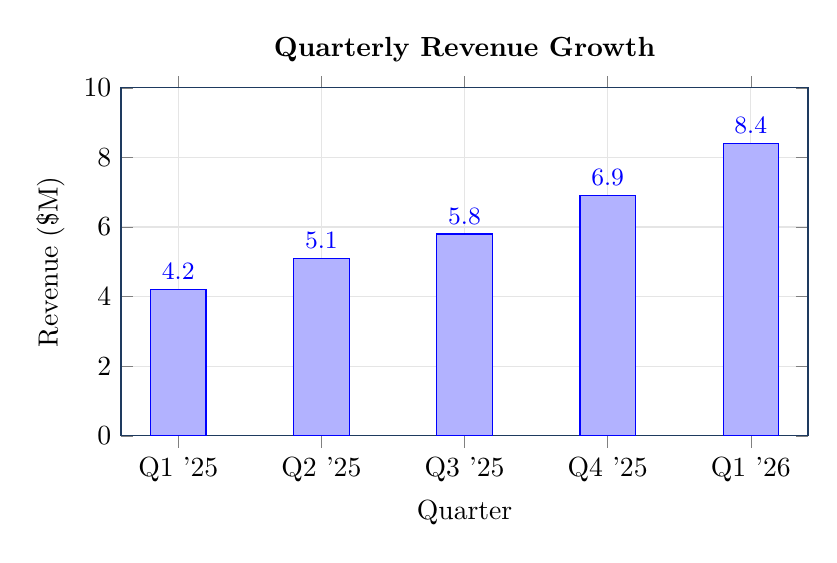
\begin{tikzpicture}
\begin{axis}[
    width=0.85\textwidth,
    height=6cm,
    ybar,
    bar width=20pt,
    xlabel={Quarter},
    ylabel={Revenue (\$M)},
    ymin=0, ymax=10,
    xtick=data,
    symbolic x coords={Q1 '25, Q2 '25, Q3 '25, Q4 '25, Q1 '26},
    nodes near coords,
    nodes near coords align={vertical},
    every node near coord/.append style={font=\small\bfseries},
    fill=accent!80,
    draw=brand,
    title={\textbf{Quarterly Revenue Growth}},
    grid=major,
    grid style={gray!20},
]
\addplot coordinates {(Q1 '25,4.2) (Q2 '25,5.1) (Q3 '25,5.8) (Q4 '25,6.9) (Q1 '26,8.4)};
\end{axis}
\end{tikzpicture}
\end{center}

Key highlights:
\begin{itemize}[leftmargin=1.5em]
    \item \textbf{Revenue}: \$8.4M (+23\% YoY), driven by Enterprise AI products
    \item \textbf{Gross Margin}: 74.2\%, up from 68.5\% in Q1 2025
    \item \textbf{New Customers}: 186 accounts, including 12 enterprise deals
    \item \textbf{Team}: 94 employees (+18 net new hires)
\end{itemize}

% ============================
% FINANCIAL PERFORMANCE
% ============================
\section{Financial Performance}

\subsection{Revenue by Segment}

\begin{table}[H]
    \centering
    \caption{Revenue breakdown by segment (USD thousands).}
    \sisetup{table-format=4.0, group-separator={,}}
    \begin{tabular}{l S S S[table-format=2.0] }
        \toprule
        \textbf{Segment} & {\textbf{Q1 2025}} & {\textbf{Q1 2026}} & {\textbf{Growth (\%)}} \\
        \midrule
        Enterprise AI    & 1800 & 3200 & 78 \\
        Platform SaaS    & 1400 & 2100 & 50 \\
        Consulting       & 600  & 1800 & 200 \\
        Data Services    & 400  & 1300 & 225 \\
        \midrule
        \textbf{Total}   & \bfseries 4200 & \bfseries 8400 & \bfseries 100 \\
        \bottomrule
    \end{tabular}
\end{table}

\subsection{Profitability Trend}

\begin{center}
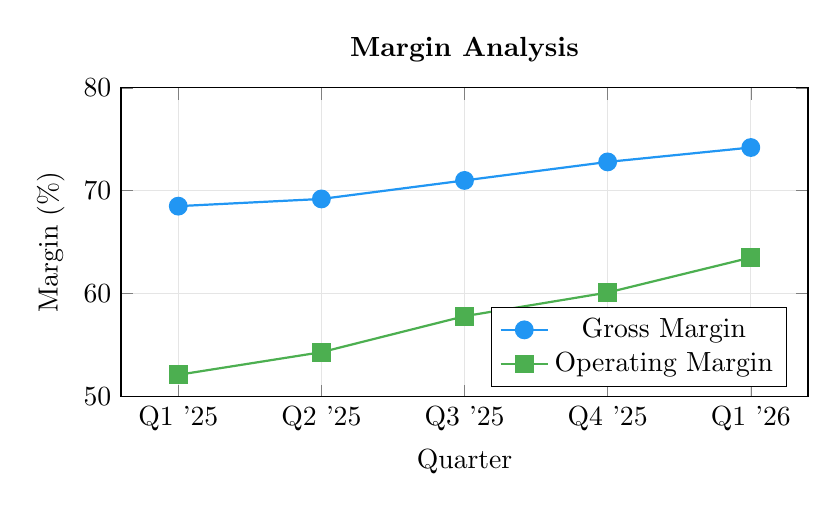
\begin{tikzpicture}
\begin{axis}[
    width=0.85\textwidth,
    height=5.5cm,
    xlabel={Quarter},
    ylabel={Margin (\%)},
    ymin=50, ymax=80,
    xtick=data,
    symbolic x coords={Q1 '25, Q2 '25, Q3 '25, Q4 '25, Q1 '26},
    legend pos=south east,
    grid=major,
    grid style={gray!20},
    title={\textbf{Margin Analysis}},
]
\addplot[color=accent,mark=*,thick,mark size=3pt] coordinates {(Q1 '25,68.5) (Q2 '25,69.2) (Q3 '25,71.0) (Q4 '25,72.8) (Q1 '26,74.2)};
\addlegendentry{Gross Margin}
\addplot[color=success,mark=square*,thick,mark size=3pt] coordinates {(Q1 '25,52.1) (Q2 '25,54.3) (Q3 '25,57.8) (Q4 '25,60.1) (Q1 '26,63.5)};
\addlegendentry{Operating Margin}
\end{axis}
\end{tikzpicture}
\end{center}

% ============================
% PRODUCT
% ============================
\section{Product \& Engineering}

\subsection{Key Releases}

\begin{table}[H]
    \centering
    \caption{Major product releases in Q1 2026.}
    \begin{tabularx}{\textwidth}{llX}
        \toprule
        \textbf{Release} & \textbf{Date} & \textbf{Impact} \\
        \midrule
        AI Agent v3.0 & Jan 18 & Autonomous task completion, 4x throughput \\
        Analytics Pro & Feb 5 & Real-time dashboards, custom KPI tracking \\
        API Gateway 2.0 & Mar 1 & GraphQL support, 200ms p99 latency \\
        Mobile SDK & Mar 15 & iOS + Android, offline mode, biometric auth \\
        \bottomrule
    \end{tabularx}
\end{table}

\subsection{Engineering Velocity}

\begin{center}
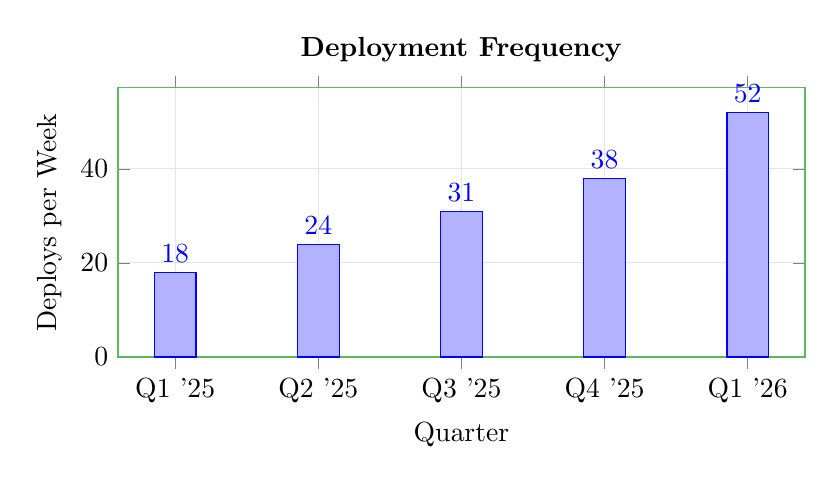
\begin{tikzpicture}
\begin{axis}[
    width=0.85\textwidth,
    height=5cm,
    ybar,
    bar width=15pt,
    xlabel={Quarter},
    ylabel={Deploys per Week},
    ymin=0,
    xtick=data,
    symbolic x coords={Q1 '25, Q2 '25, Q3 '25, Q4 '25, Q1 '26},
    nodes near coords,
    fill=success!70,
    draw=success!90,
    title={\textbf{Deployment Frequency}},
    grid=major,
    grid style={gray!20},
]
\addplot coordinates {(Q1 '25,18) (Q2 '25,24) (Q3 '25,31) (Q4 '25,38) (Q1 '26,52)};
\end{axis}
\end{tikzpicture}
\end{center}

% ============================
% MARKET POSITION
% ============================
\section{Market Position}

\begin{center}
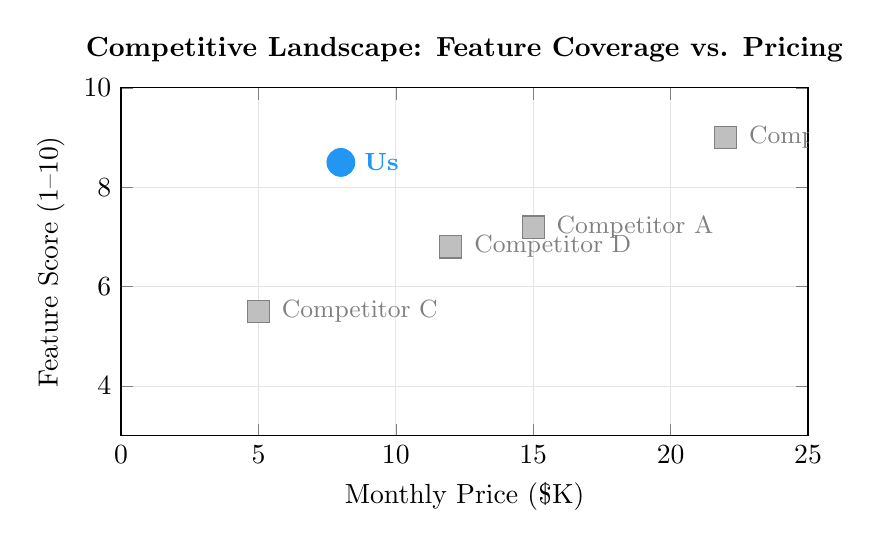
\begin{tikzpicture}
\begin{axis}[
    width=0.85\textwidth,
    height=6cm,
    title={\textbf{Competitive Landscape: Feature Coverage vs. Pricing}},
    xlabel={Monthly Price (\$K)},
    ylabel={Feature Score (1--10)},
    xmin=0, xmax=25,
    ymin=3, ymax=10,
    grid=major,
    grid style={gray!20},
    scatter/classes={
        us={mark=*,draw=accent,fill=accent,mark size=5pt},
        comp={mark=square*,draw=gray,fill=gray!50,mark size=4pt}
    },
]
\addplot[scatter,only marks,scatter src=explicit symbolic]
    coordinates {
        (8,8.5)  [us]
        (15,7.2) [comp]
        (22,9.0) [comp]
        (5,5.5)  [comp]
        (12,6.8) [comp]
    };
\node[anchor=west,font=\small\bfseries,color=accent] at (axis cs:8.5,8.5) {Us};
\node[anchor=west,font=\small,color=gray] at (axis cs:15.5,7.2) {Competitor A};
\node[anchor=west,font=\small,color=gray] at (axis cs:22.5,9.0) {Competitor B};
\node[anchor=west,font=\small,color=gray] at (axis cs:5.5,5.5) {Competitor C};
\node[anchor=west,font=\small,color=gray] at (axis cs:12.5,6.8) {Competitor D};
\end{axis}
\end{tikzpicture}
\end{center}

% ============================
% RISKS
% ============================
\section{Risks \& Mitigation}

\begin{table}[H]
    \centering
    \caption{Key risks and mitigation strategies.}
    \begin{tabularx}{\textwidth}{l l X}
        \toprule
        \textbf{Risk} & \textbf{Likelihood} & \textbf{Mitigation} \\
        \midrule
        Market slowdown & Medium & Multi-year contracts, diversified verticals \\
        Talent attrition & Low & Retention packages, equity refresh program \\
        Regulatory changes & Medium & Compliance team hired, proactive engagement \\
        Technical debt & Low & 20\% sprint allocation to infrastructure \\
        \bottomrule
    \end{tabularx}
\end{table}

% ============================
% OUTLOOK
% ============================
\section{Q2 2026 Outlook}

\begin{enumerate}
    \item \textbf{Revenue target}: \$9.8M (+17\% QoQ)
    \item \textbf{Product}: Ship AI Agent v4.0 with multi-modal support
    \item \textbf{Team}: Hire 12 engineers, 6 sales
    \item \textbf{Market}: Launch EMEA operations from London office
\end{enumerate}

\vspace{1cm}
\begin{center}
\colorbox{brand!10}{%
\begin{minipage}{0.9\textwidth}
\vspace{0.5cm}
\centering
\textcolor{brand}{\Large\textbf{Bottom Line}}\\[0.3cm]
\large Q1 exceeded all targets. The AI pivot is working.\\Revenue doubled YoY. Margins expanding. Team growing.\\The question is no longer ``if'' but ``how fast.''
\vspace{0.5cm}
\end{minipage}%
}
\end{center}

\end{document}
